\documentclass[11pt,a4paper]{report}

%%% Работа с русским языком
\usepackage{cmap}					% поиск в PDF
\usepackage{mathtext} 				% русские буквы в фомулах
\usepackage[T2A]{fontenc}			% кодировка
\usepackage[utf8]{inputenc}			% кодировка исходного текста
\usepackage[english,russian]{babel}	% локализация и переносы

\usepackage{fancyhdr}

\usepackage{lipsum}
\usepackage{etoolbox}

% Code in Latex
\usepackage{listings}

%%% Работа с картинками
\usepackage{graphicx}  % Для вставки рисунков
%\graphicspath{{images/}}  % папки с картинками
\setlength\fboxsep{3pt} % Отступ рамки \fbox{} от рисунка
\setlength\fboxrule{1pt} % Толщина линий рамки \fbox{}
\usepackage{wrapfig} % Обтекание рисунков и таблиц текстом
\usepackage[export]{adjustbox}

%%% Дополнительная работа с математикой
\usepackage{amsmath,amsfonts,amssymb,amsthm,mathtools} % AMS
\usepackage{icomma} % "Умная" запятая: $0,2$ --- число, $0, 2$ --- перечисление
\usepackage{systeme}

\usepackage{tabularx}
\usepackage{tikz-cd}

%%% Работа с картинками
\usepackage{graphicx}  % Для вставки рисунков
%\graphicspath{{images/}}  % папки с картинками
\setlength\fboxsep{3pt} % Отступ рамки \fbox{} от рисунка
\setlength\fboxrule{1pt} % Толщина линий рамки \fbox{}
\usepackage{wrapfig} % Обтекание рисунков и таблиц текстом
\usepackage[export]{adjustbox}

\patchcmd{\maketitle}
  {\end{titlepage}}
  {\thispagestyle{titlepagestyle}\end{titlepage}}
  {}{}

\fancypagestyle{titlepagestyle}
{
   \fancyhf{}
   \fancyfoot[C]{3 курс, 3 группа}
   \renewcommand{\headrulewidth}{0 mm}
}

\pagestyle{plain}

\begin{document}
	
\lstset{ 
	language=Python, 
	tabsize=2, 
	showspaces=false, 
	showstringspaces=false, 
	float=[htb], 
	captionpos=b, 
	basicstyle=\footnotesize,
	numberblanklines=false, 
} 



\title{Отчет по лабораторной работе №4}

\author{Снопов П.М.}
\thispagestyle{titlepagestyle}
\maketitle
\begin{center}
	\textbf{Лабораторная работа №4}
	
	Решение задачи Коши для ОДУ 1-ого порядка методами Рунге-Кутта. 
	
	\textit{Задача 11; Вариант 3}
\end{center}

\paragraph{1. Постановка задачи}
Решение задачи Коши с заданной точностью с автоматическим выбором максимальной длины шага:

Имеется обыкновенное дифференциальное уравнение $ y' = f(x,y) $, где $ x \in [A, B] $ с начальным условием $ y(C) = y_c $, где $ С \in \{A,B\} $. Необходимо численно решить ОДУ с заданной точностью и автоматическим выбором длины шага.
\paragraph{2. Метод решения}
Решать задачу будем методом Рунге-Кутта второго порядка, для уточнения решения будем пользоваться методом Рунге-Кутта четвертого порядка. Явный метод Рунге-Кутта задается формулами:
\[
\begin{aligned}
&y_{n+1} = y_n + h\sum_{i=1}^s b_ik_i \\
&k_1 = f(x_n, y_n)\\
&k_2 = f(x_n + c_2h, y_n + a_{21}hk_1)\\
&...\\
&k_s = f(x_n + c_sh, y_n+\sum_{p=1}^{s-1} a_{sp}hk_p)
\end{aligned}.
\]

Где h -- величина шага сетки по $ x $.

Для решения данной задачи воспользуемся следующим методом второго порядка:
\[
\begin{aligned}
&y_{n+1} = y_n + k_2\\
&k_1 = hf(x_n,y_n)\\
&k2 = hf(x_n + \frac{1}{2}h, y_n + \frac{1}{2}k_1)
\end{aligned}
\]

А для уточнения данной задачи воспользуемся следующим методом четвертого порядка:
\[
\begin{aligned}
&y_{n+1} = y_n + \frac{1}{6}(k_1 + 2k_2 + 2k_3 + k_4)\\
&k_1 = hf(x_n,y_n)\\
&k_2 = hf(x_n + \frac{1}{2}h, y_n + \frac{1}{2}k_1)\\
&k_3 = hf(x_n + \frac{1}{2}h, y_n + \frac{1}{2}k_2)\\
&k_4 = hf(x_n + h, y_n + k_3)
\end{aligned}
\]
Для начала пусть $ h := \frac{B - A}{10} $. Далее на каждом шагу определяем рекомендуемую длину шага следующим образом:
\[
h_e := \sqrt[\leftroot{-2}\uproot{5}\frac{1}{4}]{\frac{\varepsilon_n}{\varepsilon}}h
\]
где $ \varepsilon_n := |\hat{y}_n - \tilde{y}_n | $, где $\hat{y}_n$ -- значение, полученное методом второго порядка, а $\tilde{y}_n$-- методом четвертого порядка. Далее проводим выбор шага следующим образом:

\[
h_n = \begin{cases}
	h_{min}, & \text{если $h_e < h_{min}$} \\
	h_e, & \text{если $h_{min} < h_e < h_{max}$} \\
	h_{max}, & \text{если $h_e > h_{max}$}
\end{cases}
\]

\paragraph{3. Основные процедуры}
Основные функции, используемые при решении задачи:


\begin{lstlisting}
def estimate(f: Callable, h: float, x: float, y=0) -> float:
\end{lstlisting}
Функция, соответствующая методу Рунге-Кутта второго порядка
\begin{lstlisting}
def optimize(f: Callable, h: float, x: float, y=0) -> float:
\end{lstlisting}
Функция, соответствующая методу Рунге-Кутта четвертого порядка
\begin{lstlisting}
def get_data(name: str) -> list:
\end{lstlisting}
Функция для получения данных
\begin{lstlisting}
def give_data(X:list, Y:list):
\end{lstlisting}
Функция записывающая полученные данные
\begin{lstlisting}
def solve(f: Callable) -> list:
\end{lstlisting}
Основная функция, осуществляющая решение задачи.
\paragraph{3. Графики полученного численного решения и точного}
\begin{figure}[h!]
	\centering
	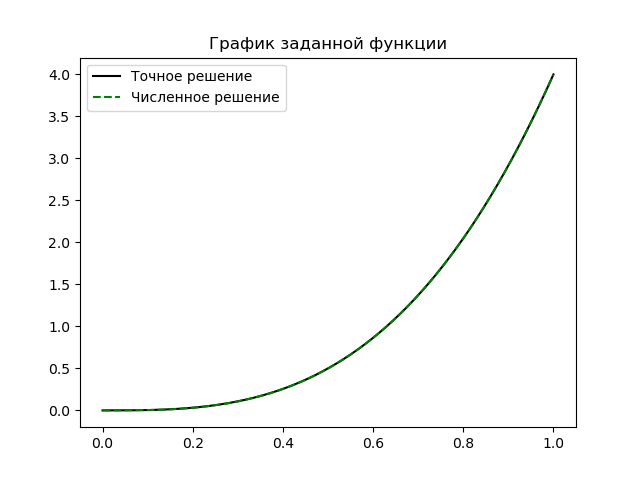
\includegraphics[width=\linewidth, keepaspectratio=true]{graphs.png}
	\caption{Графики}
	\label{fig:jobs}
\end{figure}
\end{document}